\documentclass{beamer}
\usepackage[utf8]{inputenc}

\usetheme{Madrid}
\usecolortheme{default}
\usepackage{amsmath,amssymb,amsfonts,amsthm}
\usepackage{txfonts}
\usepackage{tkz-euclide}
\usepackage{listings}
\usepackage{adjustbox}
\usepackage{array}
\usepackage{tabularx}
\usepackage{gvv}
\usepackage{lmodern}
\usepackage{circuitikz}
\usepackage{tikz}
\usepackage{graphicx}

\setbeamertemplate{page number in head/foot}[totalframenumber]

\usepackage{tcolorbox}
\tcbuselibrary{minted,breakable,xparse,skins}



\definecolor{bg}{gray}{0.95}
\DeclareTCBListing{mintedbox}{O{}m!O{}}{%
  breakable=true,
  listing engine=minted,
  listing only,
  minted language=#2,
  minted style=default,
  minted options={%
    linenos,
    gobble=0,
    breaklines=true,
    breakafter=,,
    fontsize=\small,
    numbersep=8pt,
    #1},
  boxsep=0pt,
  left skip=0pt,
  right skip=0pt,
  left=25pt,
  right=0pt,
  top=3pt,
  bottom=3pt,
  arc=5pt,
  leftrule=0pt,
  rightrule=0pt,
  bottomrule=2pt,
  toprule=2pt,
  colback=bg,
  colframe=orange!70,
  enhanced,
  overlay={%
    \begin{tcbclipinterior}
    \fill[orange!20!white] (frame.south west) rectangle ([xshift=20pt]frame.north west);
    \end{tcbclipinterior}},
  #3,
}
\lstset{
    language=C,
    basicstyle=\ttfamily\small,
    keywordstyle=\color{blue},
    stringstyle=\color{orange},
    commentstyle=\color{green!60!black},
    numbers=left,
    numberstyle=\tiny\color{gray},
    breaklines=true,
    showstringspaces=false,
}
%------------------------------------------------------------

\title
{2.10.23}
\author 
{AI25BTECH11034 - Sujal Chauhan }



\begin{document}

\frame{\titlepage}
\begin{frame}{Question}

The vector(s) which is/are coplanar with the vectors $\hat{i}+\hat{j}+2\hat{k}$ and $\hat{i}+2\hat{j}+\hat{k}$, and perpendicular to vector $\hat{i}+\hat{j}+\hat{k}$ is/are.
\begin{enumerate}
    \item $\hat{\mathbf{j}} - \hat{\mathbf{k}}$
    \item $\hat{\mathbf{i}} + \hat{\mathbf{j}}$
    \item $\hat{\mathbf{i}} - \hat{\mathbf{j}}$
    \item $\hat{\mathbf{j}} + \hat{\mathbf{k}}$
\end{enumerate}
\end{frame}


\begin{frame}{Solution}
\begin{center}
\begin{tabular}{|c|c|}
\hline
Variable & Vector \\ \hline
$\vec{A}$ & $\myvec{1 \\ 1 \\ 2}$ \\ \hline
$\vec{B}$ & $\myvec{1 \\ 2 \\ 1}$ \\ \hline
$\vec{C}$ & $\myvec{1 \\ 1 \\ 1}$ \\ \hline
\end{tabular}
\end{center}
\end{frame}
\begin{frame}{Solution}
Listing options as vectors $\vec{D_i}$:

\begin{center}
\begin{tabular}{|c|c|}
\hline
Input & Vector \\ \hline
$\vec{D_1}$ & $\myvec{0 \\ 1 \\ -1}$ \\ \hline
$\vec{D_2}$ & $\myvec{1 \\ 1 \\ 1}$ \\ \hline
$\vec{D_3}$ & $\myvec{1 \\ -1 \\ 0}$ \\ \hline
$\vec{D_4}$ & $\myvec{0 \\ 1 \\ 1}$ \\ \hline
\end{tabular}
\end{center}
\end{frame}

\begin{frame}{Checking conditions}

Let equation of plane be given by:
\begin{align}
    \vec{n}^\top\vec{X}=1
\end{align}
Let's find general solution $\vec{n}$ which is perpendicular to the plane 
\begin{align}
    \myvec{A && B}^\top\vec{n}=\myvec{1 \\ 1}
\end{align}
\begin{align}
&\text{Given:} \quad
  \myvec{1 & 1 & 2\\ 1 & 2 & 1}\vec{n} = \myvec{1 \\ 1} \\[1em]
\end{align}
\end{frame}
\begin{frame}
\begin{align}
&\text{We want to solve:} \quad 
\myvec{1 & 1 & 2 \\ 1 & 2 & 1}\vec{n} = \myvec{1 \\ 1}, 
\quad \vec{n} = \myvec{n_1 \\ n_2 \\ n_3} 
\end{align}

\begin{align}
&\text{Form the augmented matrix:} \\
&\myvec{1 & 1 & 2 & \vline & 1 \\ 1 & 2 & 1 & \vline & 1}
\end{align}

\begin{align}
&\xrightarrow{R_2 \to R_2 - R_1}
\myvec{1 & 1 & 2 & \vline & 1 \\ 0 & 1 & -1 & \vline & 0}
\end{align}

\begin{align}
&\xrightarrow{R_1 \to R_1 - R_2}
\myvec{1 & 0 & 3 & \vline & 1 \\ 0 & 1 & -1 & \vline & 0}
\end{align}
\end{frame}
\begin{frame}
\begin{align}
&\text{Thus the equations are:} \\
&n_1 + 3n_3 = 1, \quad n_2 - n_3 = 0
\end{align}

\begin{align}
&\text{Let } n_3 = a \in \mathbb{R}, \quad
n_2 = a, \quad n_1 = 1 - 3a
\end{align}

\begin{align}
&\text{So the general solution is:} \\
&\vec{n} = \myvec{1 - 3a \\ a \\ a}, \quad a \in \mathbb{R}
\end{align}
\end{frame}
\begin{frame}

Now any vector following both condition will be solution of the equation:
\begin{align}
    \myvec{ n & C}^\top\vec{D_i}=\myvec{0\\0}
\end{align}
Checking Values for all options:
\begin{align}
    \myvec{1-3a & a & a \\ 1 & 1 &1}\vec{D_i}=\myvec{0 \\ 0}
\end{align}
\end{frame}
\begin{frame}
\begin{center}
\begin{tabular}{|c|c|c|}
\hline
Vector & $ \myvec{1-3a & a & a \\ 1 & 1 &1}\vec{D_i}$ & Satisfies\\ \hline
$\vec{D_1}$ & $\myvec{0\\0}$ & Yes \\ \hline
$\vec{D_2}$ & $\myvec{1-2a\\2}$  & No  \\ \hline
$\vec{D_3}$ & $\myvec{1-4a\\0}$ & No \\ \hline
$\vec{D_4}$ & $\myvec{2a\\2}$  & No  \\ \hline
\end{tabular}
\end{center}

So only $\vec{D_1}$ satisfies both conditions.




\end{frame}
\begin{frame}{figure}
\begin{figure}[H]
    \centering
    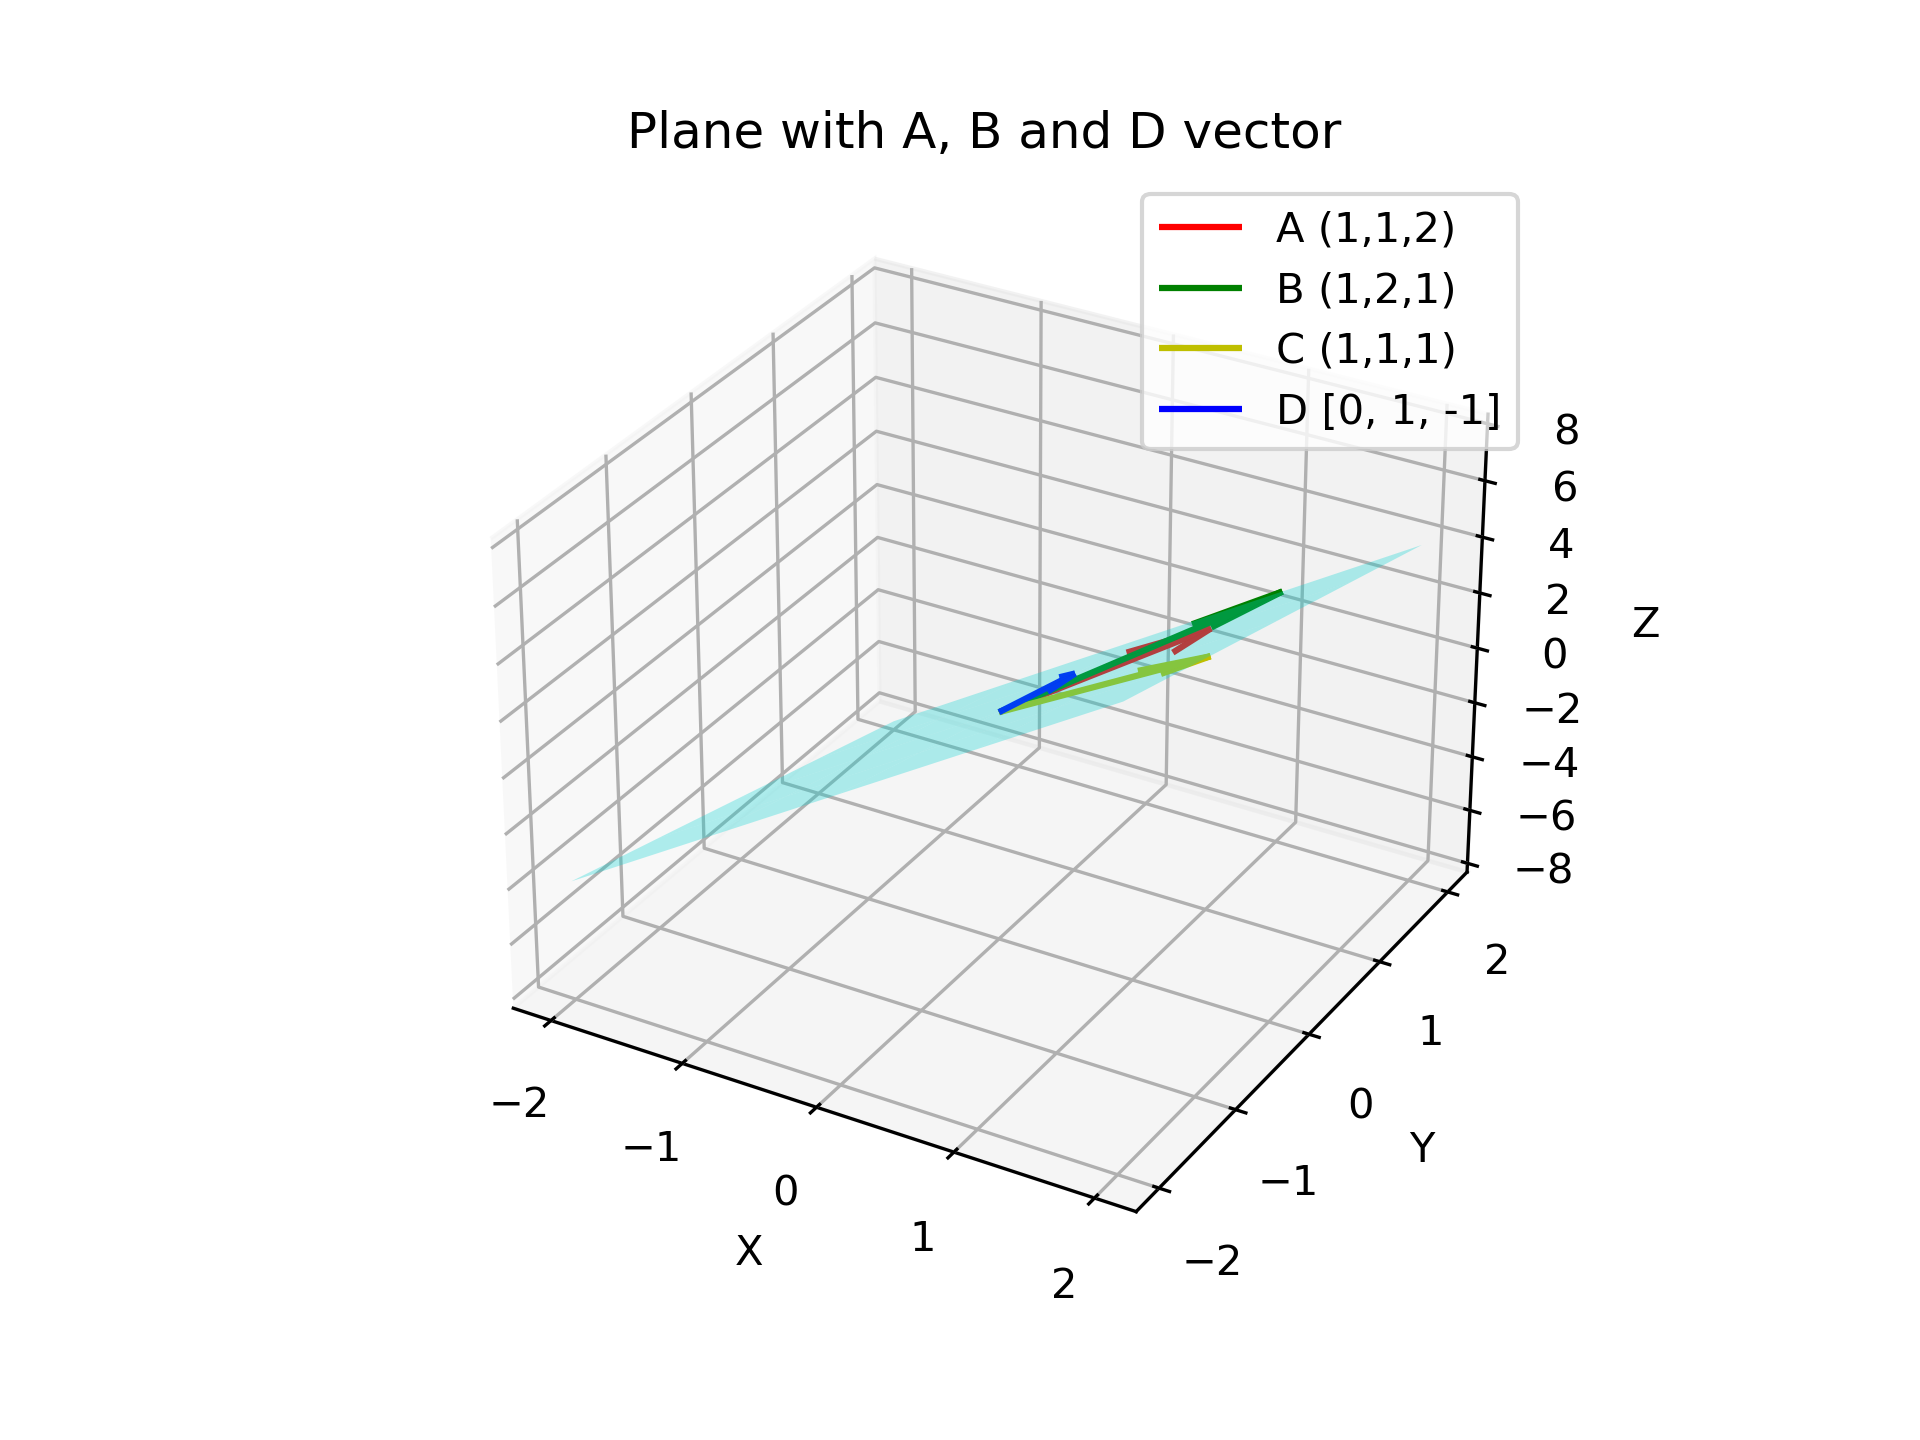
\includegraphics[width=0.6\linewidth]{figures/plane_1.png}
    \caption{Vector $\vec{D_1}$ in plane}
\end{figure}
\end{frame}
\begin{frame}{figure}
\begin{figure}[H]
    \centering
    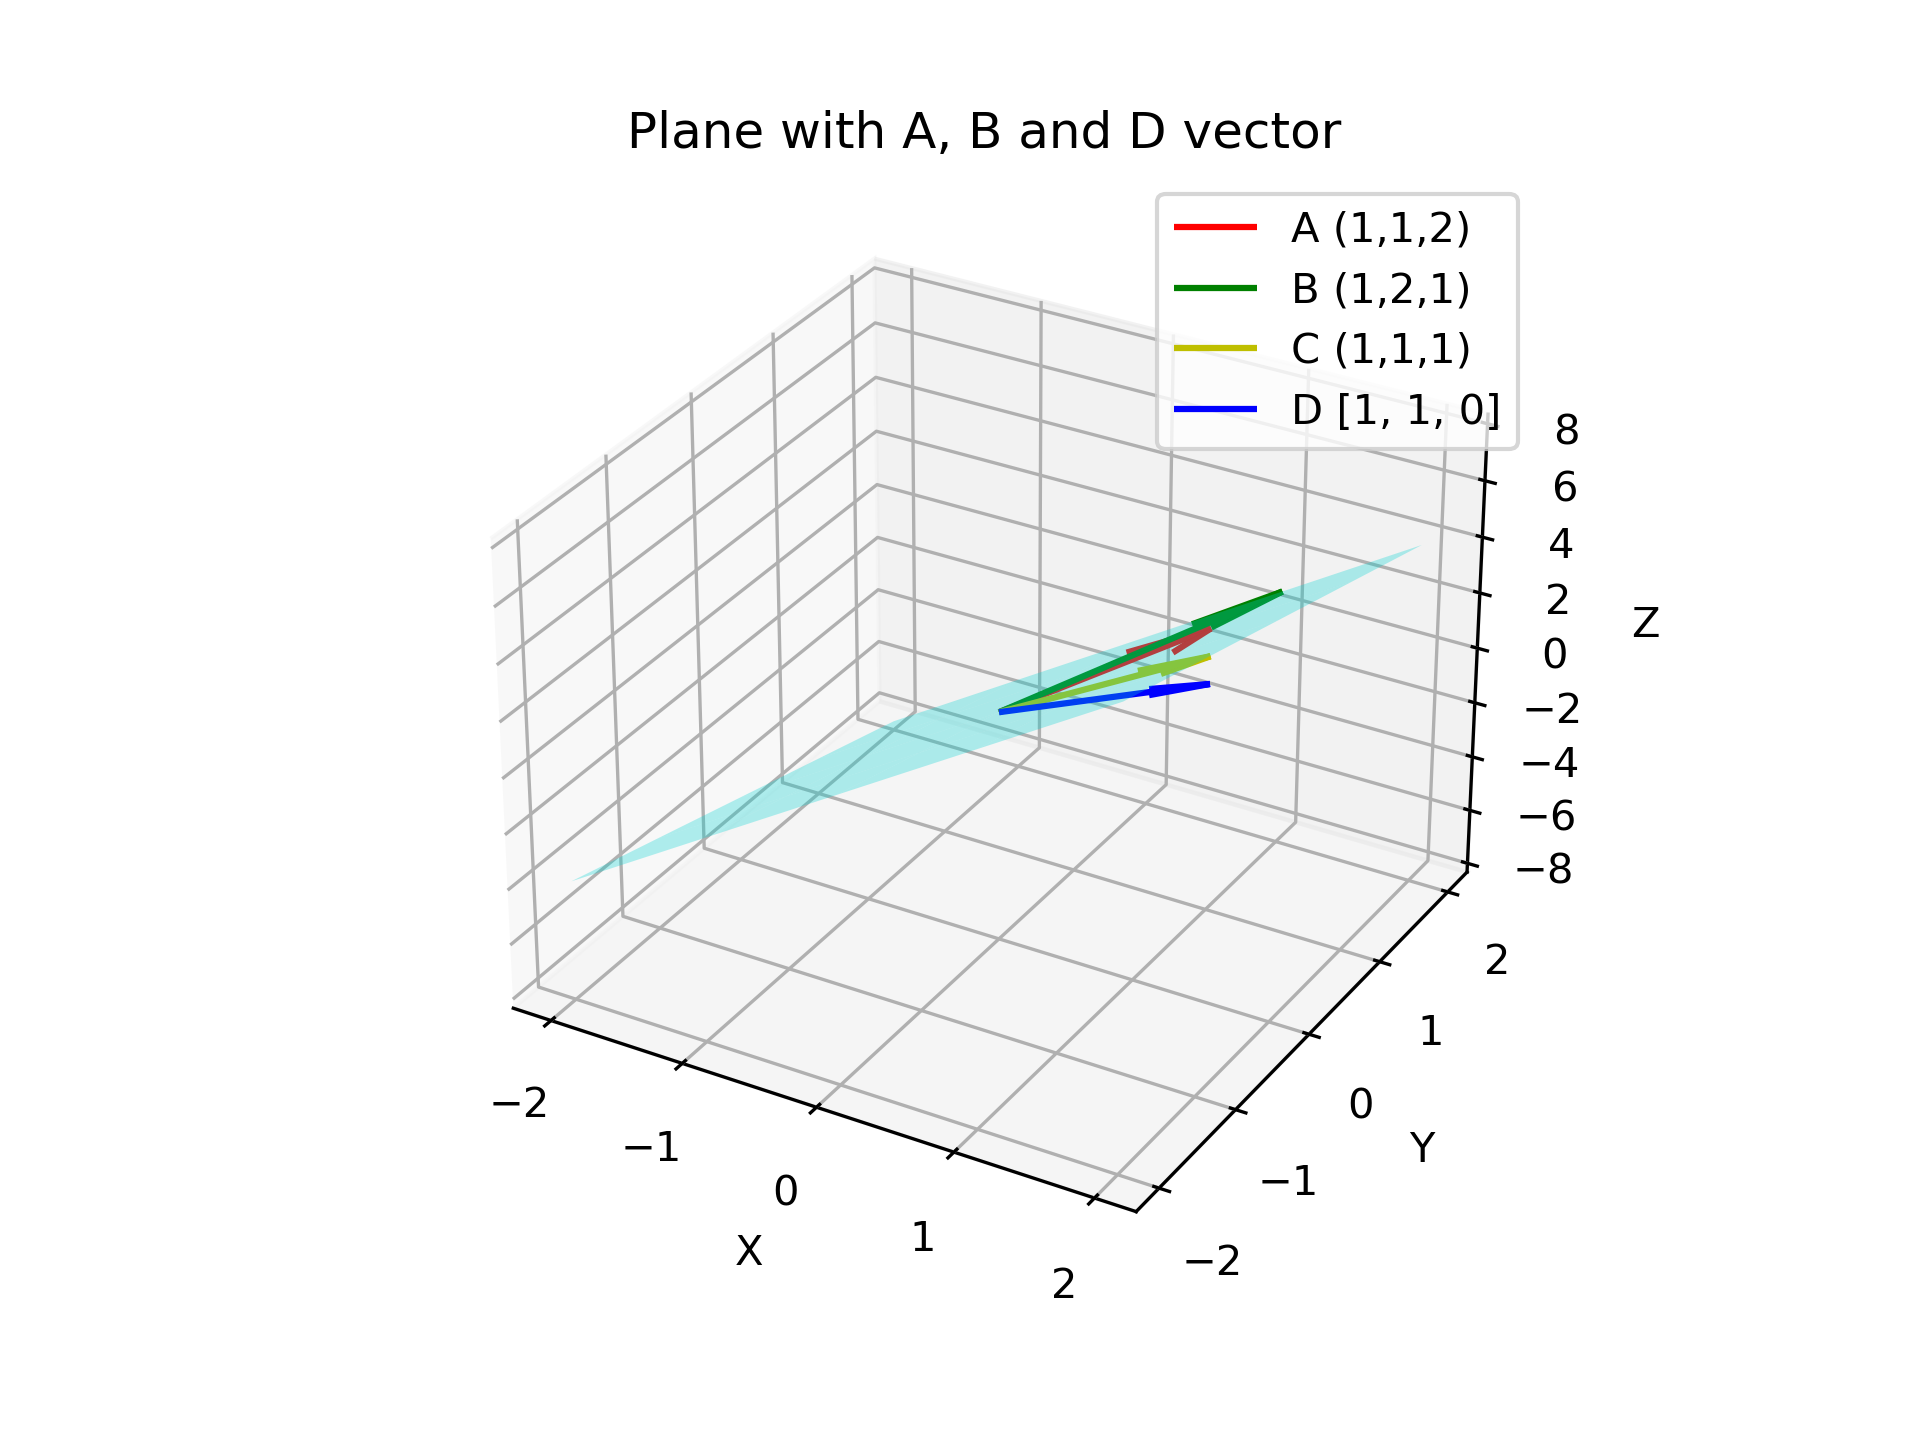
\includegraphics[width=0.6\linewidth]{figures/plane_2.png}
    \caption{Vector $\vec{D_2}$ not coplanar}
\end{figure}
\end{frame}
\begin{frame}{figure}
\begin{figure}[H]
    \centering
    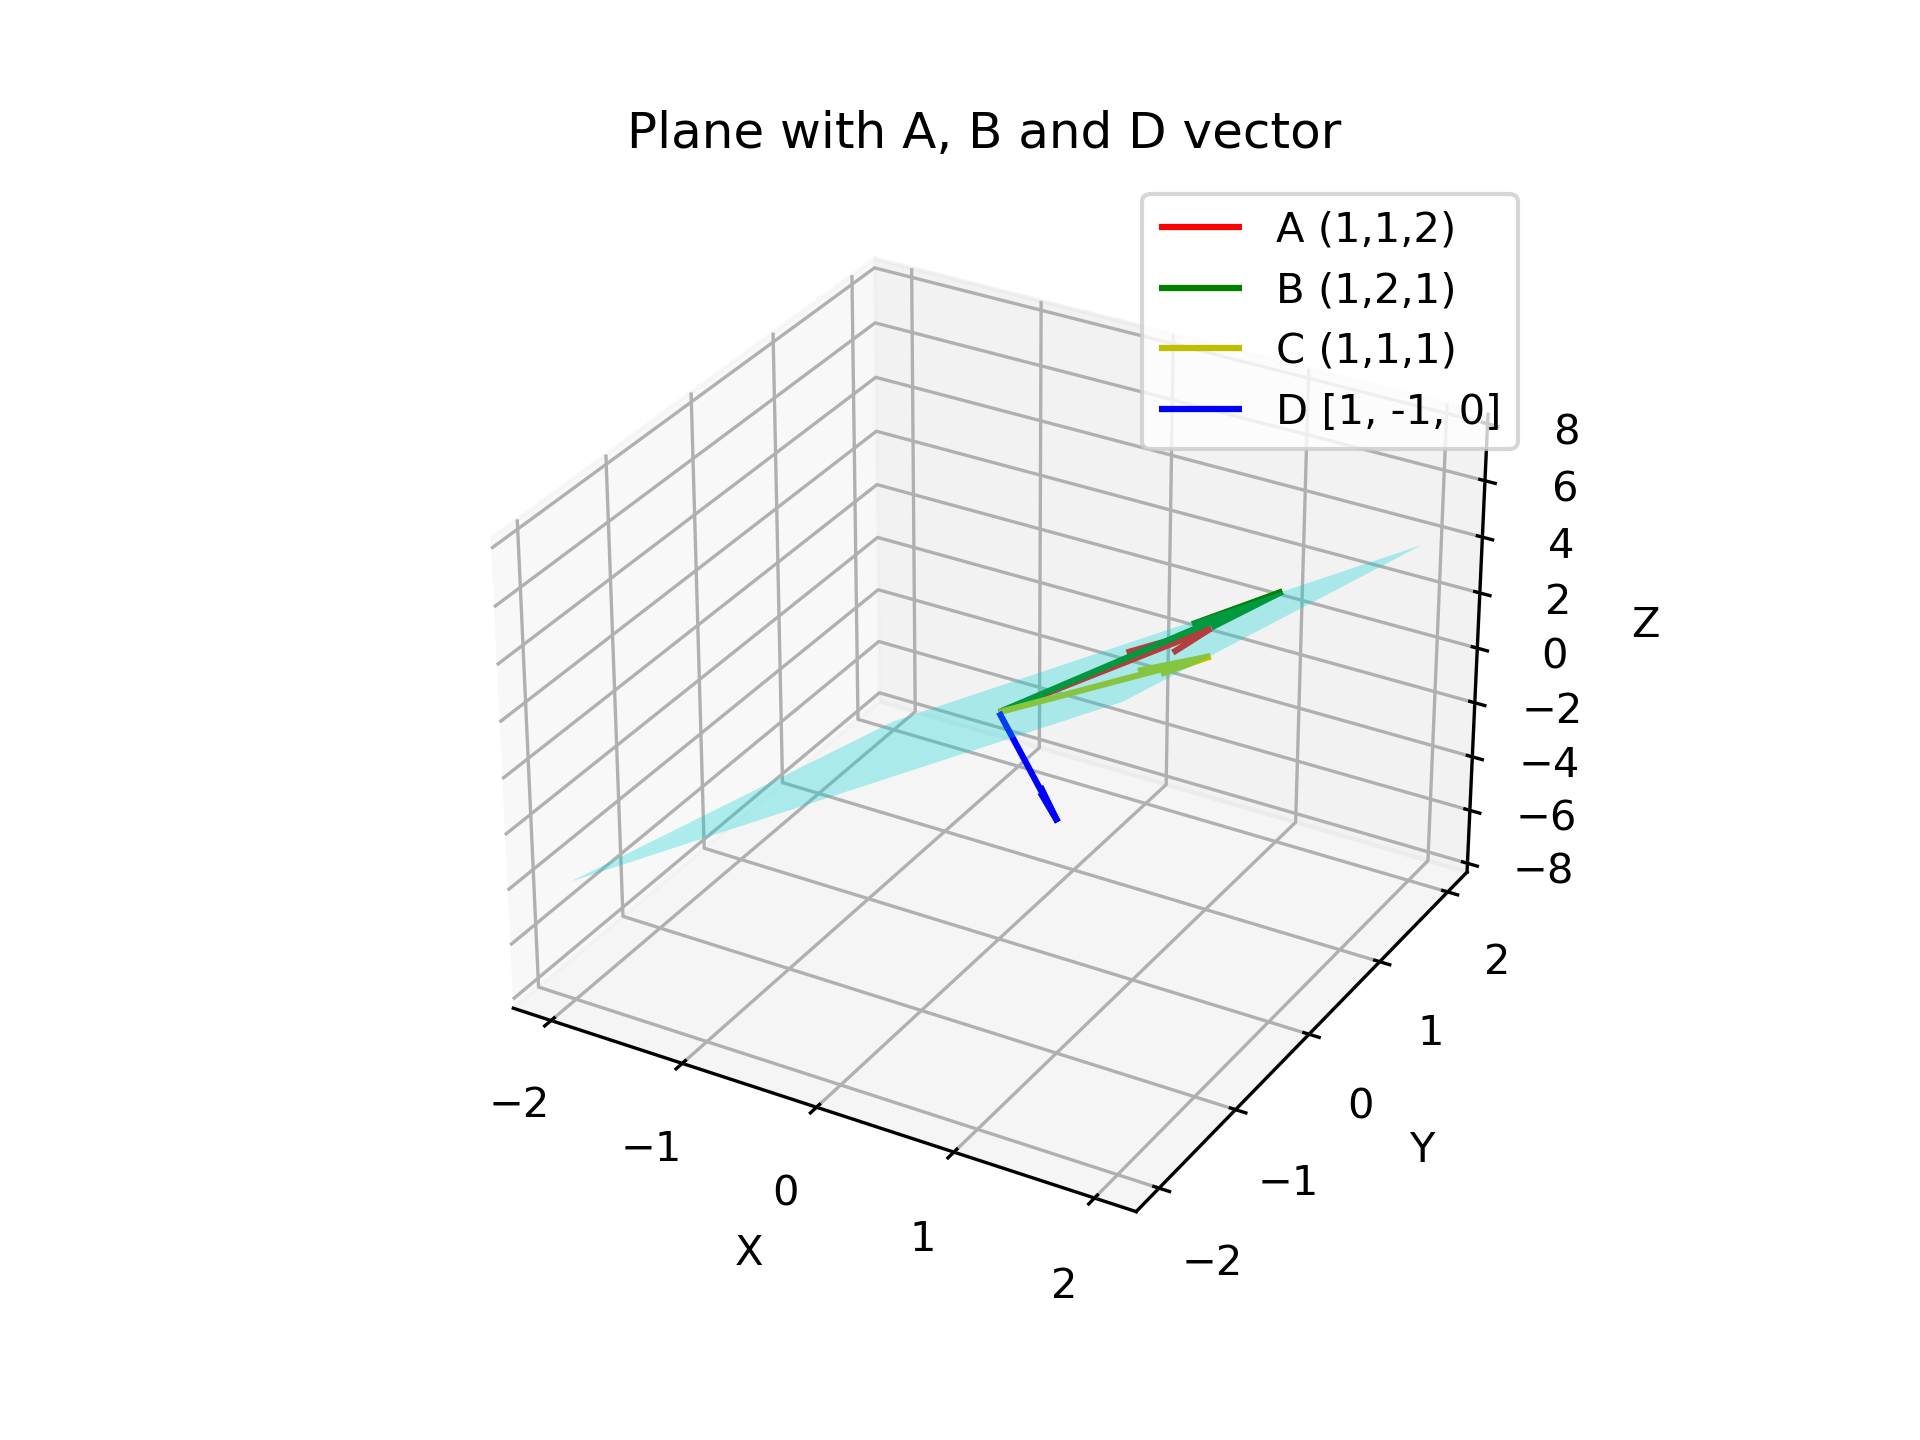
\includegraphics[width=0.6\linewidth]{figures/plane_3.png}
    \caption{Vector $\vec{D_3}$ not coplanar}
\end{figure}
\end{frame}
\begin{frame}{figure}
\begin{figure}[H]
    \centering
    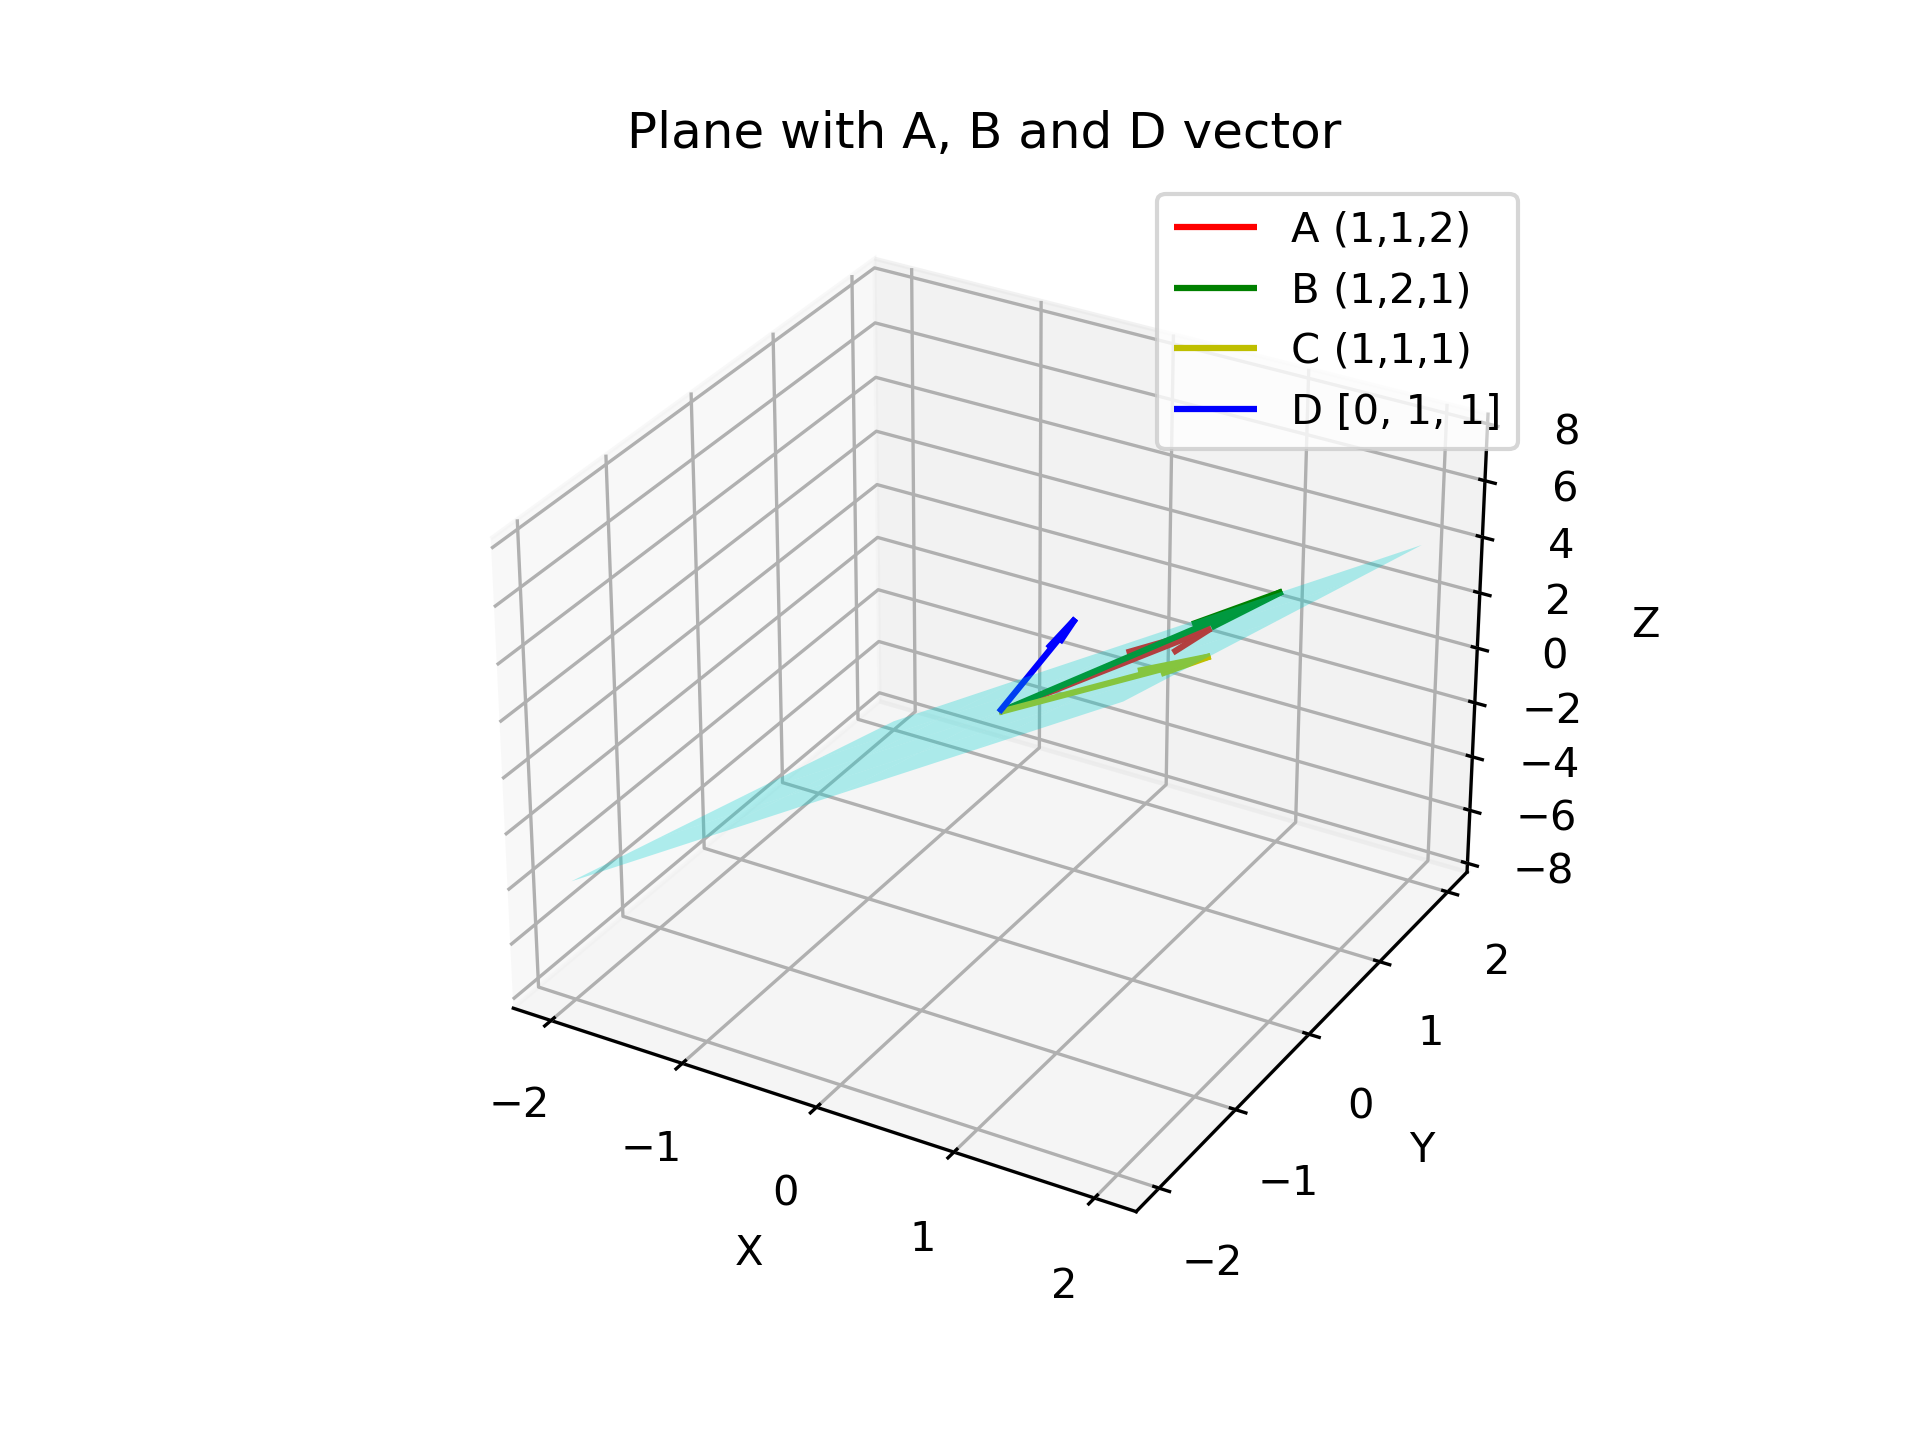
\includegraphics[width=0.6\linewidth]{figures/plane_4.png}
    \caption{Vector $\vec{D_4}$ not coplanar}
\end{figure}
\end{frame}
\begin{frame}{conclusion}
\textbf{\Large Only 1 satisfys both conditions}
\end{frame}





\end{document}
